% !TeX root = ..\main.tex
\npchapter{Grundlagen} \label{ch:foundations}
Dieses Kapitel stellt die benötigten Grundlagen vor, die für das Verständnis der darauffolgenden Kapitel notwendig sind. Hierzu zählen die Vorstellung von Node.js und Bun sowie weitere Grundlagen zu Performanceanalysen.

\section{Node.js} \label{sec:foundations-Node.js}
Node.js ist ein beliebtes Tool für eine Vielzahl an unterschiedlichen Projekten, darunter leichtgewichtige Webservices, dynamische Webanwendungen und Tools für die Kommandozeile. Es handelt sich um eine plattformunabhängige Open-Source-Laufzeitumgebung, die es ermöglicht, JavaScript außerhalb des Browsers auszuführen. Node.js verwendet die V8 JavaScript Engine von Google. Diese ist in C++ geschrieben und wird von Google Chrome verwendet. Dies ermöglicht Node.js eine hohe Performance, weshalb Unternehmen wie Netflix und Uber Node.js in ihren Softwareprojekten einsetzen.\cite{OpenJSFoundation.2022}\\

\begin{figure}[h]
	\centering
	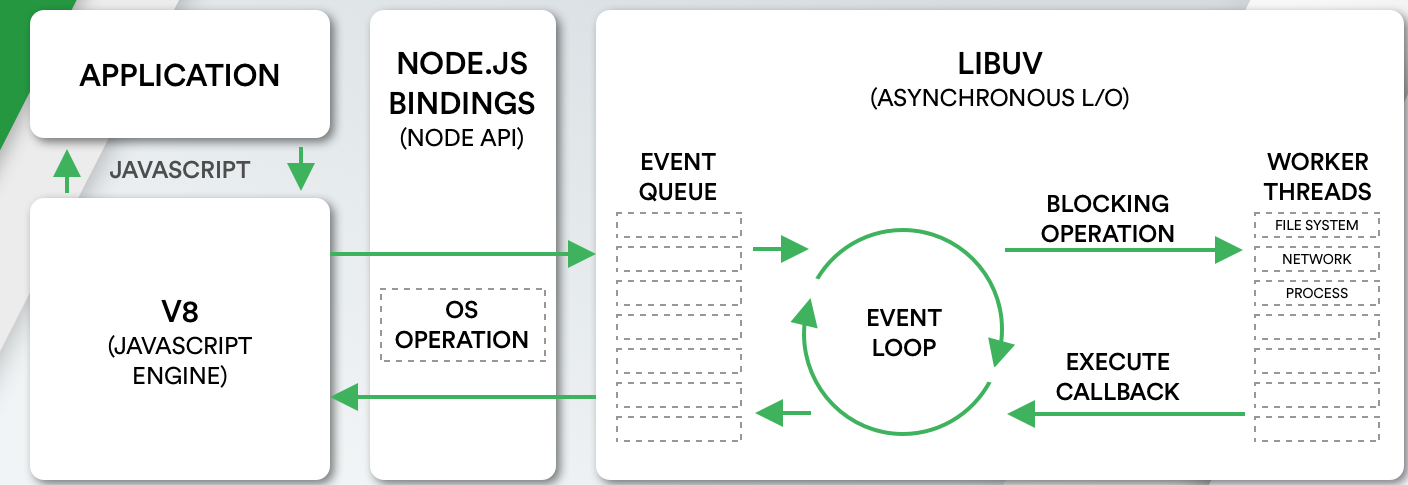
\includegraphics[width=\linewidth]{./images/NodeJsArchitecture}
	\caption{Node.js Architektur}
	\label{fig:nodejsArchitecture}
	\textit{Quelle: \cite{Kaneriya.2022}}
\end{figure}
 
\noindent
Wie in \autoref{fig:nodejsArchitecture} zu sehen, nutzt Node.js grundsätzlich nur einen Thread und erstellt nicht für jede neue Anfrage einen neuen Thread. Sobald eine Applikation gestartet wird, wird in dem einzigen Thread der Node.js-Prozess gestartet. Die V8 Engine optimiert den Maschinencode zusätzlich an häufig benötigten Stellen, wobei dies nicht sofort geschieht, da die Übersetzung in Maschinencode aufgrund der Just-in-Time-Kompilierung eine zeitsensitive Aufgabe darstellt. Darüber hinaus ist in der Engine ein Garbage Collector integriert, der nicht mehr verwendete Objekte löscht.\cite{Springer.2022} \newline 
Für weitere Aufgaben setzt Node.js auf Bibliotheken, die fertige und etablierte Lösungsansätze für häufig benötigte Aufgaben zur Verfügung stellen. Nur für Aufgaben, für die es keine etablierte Bibliothek gibt, werden eigene Implementierungen verwendet. Im Folgenden werden die wichtigsten Komponenten vorgestellt.\cite{Springer.2022}\\

\noindent
\textbf{Node.js Bindings} \newline
Node.js Bindings, auch bekannt als Node.js Add-ons, schaffen die Möglichkeit C- oder C++-Quellcode in Node.js zu integrieren. Entwickler können Erweiterungen in nativem Code erstellen und in ihren Anwendungen in JavaScript nutzen. Dies ermöglicht die Nutzung von Systemfunktionalitäten. Dies wird beispielsweise für den Zugriff auf das Dateisystem im Modul \textit{fs} verwendet. Dieses ist in der \ac{api} von Node.js enthalten. Darin bietet Node.js viele Lösungen für häufig benötigte Aufgaben, um die Entwicklung zu vereinfachen. Diese sind global im gesamten Anwendungscode verfügbar. Zu den globalen Objekten gehören beispielsweise \textit{console} für die Ausgabe von Informationen in der Konsole und \textit{Buffer} für den Umgang mit binären Daten. In der \ac{api} ist neben dem Modul \textit{fs} beispielsweise das Modul \textit{http} enthalten, um den Umgang mit dem HTTP-Protokoll zu vereinfachen. Die Module selbst sind in JavaScript geschrieben. D. h. der Kern von Node.js liegt in C (Libuv) und C++ (V8 Engine)  vor, die übrigen Komponenten sind in der Sprache der Plattform geschrieben. Allerdings ist in der Standard-API keine Unterstützung für TypeScript enthalten. Hierzu muss der TypeScript-Transpiler separat installiert werden.\cite{Springer.2022, OpenJSFoundation.2022b, OpenJSFoundation.o.J.b}\\

\noindent
\textbf{Event Loop} \newline
Node.js verwendet eine eventgesteuerte Architektur. Anstatt den Quellcode linear auszuführen, werden definierte Events ausgelöst, für die zuvor Callback-Funktionen registriert wurden. Dieses Konzept wird genutzt, um eine hohe Anzahl von asynchronen Aufgaben zu bewältigen. Um dabei den einzelnen Thread der Anwendung nicht zu blockieren, werden Lese- und Schreiboperationen an den Event Loop ausgelagert.  Wenn auf externe Ressourcen zugegriffen werden muss, leitet der Event Loop die Anfrage weiter und die registrierte Callback-Funktion gibt die Anfrage an das Betriebssystem weiter. In der Zwischenzeit kann Node.js andere Operationen ausführen. Das Ergebnis der externen Operation wird dann über den Event Loop zurückgeliefert.\cite{Springer.2022} \newline 
Während der Laufzeit werden viele Events erzeugt und in einer Message Queue, der Event Queue, nacheinander gespeichert. Node.js nutzt First In First Out \todo{Rechtschreibung prüfen} und beginnt demnach mit der Verarbeitung der ältesten Events und arbeitet sich durch die Queue, bis keine Events mehr vorhanden sind.\cite{OpenJSFoundation.o.J.c}\\

\noindent
\textbf{Libuv}\todo{Prüfen, ob tatsächlich großes L (siehe Quelle)} \newline
Der Event Loop von Node.js basiert ursprünglich auf der Bibliothek libev. Diese ist in C geschrieben und für ihre hohe Leistung und umfangreichen Features bekannt. Allerdings stützt sich libev auf native UNIX-Funktionen. Diese sind auf Windows über eine andere Schnittstelle nutzbar. Daher dient Libuv als Abstraktionsebene zwischen Node.js und den darunter liegenden Bibliotheken für den Event Loop, um die Laufzeitumgebung auf allen Plattformen nutzen zu können. Libuv verwaltet alle asynchronen I/O-Operationen, einschließlich Dateisystemzugriffe und asynchrone TCP- und UDP-Verbindungen.\cite{Springer.2022} \\

\noindent
\textbf{\ac{npm}} \newline
Darüber hinaus bringt Node.js den \ac{npm} mit sich. Dieser Paketmanager ist entscheidend für den Erfolg von Node.js, da es im September 2022 mehr als 2,1 Millionen Pakete in diesem Ökosystem gibt. Es gibt somit ein Paket für eine Vielzahl an Anwendungsfällen. Ursprünglich wurde \ac{npm} entwickelt, um Abhängigkeiten in Projekten zu verwalten. Mittlerweile wird \ac{npm} auch als Werkzeug für JavaScript im Frontend unterstützt. \todo{Aussage in Quelle nochmal prüfen, um besser zu formulieren} Der \ac{npm} ist nicht Teil des Executables von Node.js und wird bei der Installation häufig mitgeliefert. \cite{Springer.2022, OpenJSFoundation.2022b}\\

\noindent
Zusammenfassend zeichnet sich Node.js durch eine eventgesteuerte Architektur und durch ein nicht blockierendes Modell für Ein- und Ausgabeoperationen aus. Dieser Aufbau macht es leichtgewichtig und effizient macht. Dies hat verschiedene Vor- und Nachteile. \newline
Zu den Vorteilen gehören eine hohe Performance durch die Nutzung der V8 JavaScript Engine und die Plattformunabhängigkeit. Eine weitere Stärke ist die große und aktive Community an Entwicklern. Dank der Popularität gibt es viele etablierte Lösungsansätze, die den Entwicklungsprozess beschleunigen und vereinfachen. Node.js ermöglicht die Verwendung der JavaScript-Sprache sowohl auf der Server- als auch auf der Clientseite. Dies vereinfacht die Entwicklung von Full-Stack-Anwendungen und erleichtert Entwicklern den Einstieg.\cite{Brown.November2019, OpenJSFoundation.2022b} \newline
Allerdings existieren auch Nachteile bei der Verwendung von Node.js. Das Single-Thread-Modell kann bei rechenintensiven oder CPU-lastigen Aufgaben zu Engpässen führen, da es nur einen Hauptthread für die Ausführung von Code gibt  \cite{Chhetri.2016}. Ein weiterer Nachteil ist, dass Node.js über eine begrenzte Standardbibliothek verfügt, sodass Entwickler häufig auf externe Module und Pakete zurückgreifen müssen, beispielsweise der Transpiler für TypeScript \cite{OpenJSFoundation.2022b}.

\section{Bun} \label{sec:foundations-Bun}
Bun ist ein Open-Source-Toolkit für JavaScript. Dieses kombiniert verschiedene serverseitige Komponenten, um eine leistungsstarkes Paket zur Verfügung zu stellen. Bun ist auf MacOS und Linux für die produktive Nutzung freigegeben. Die Version von Windows besitzt aktuell einen experimentellen Status und ist noch nicht für Performance optimiert. Alternativ kann auf Windows die veröffentlichte Linux-Version über das Windows Subsystem für Linux installiert werden. Ursprünglich ist Bun als ein persönliches Freizeitprojekt von Jared Sumner gestartet. Mittlerweile hat es sich zu einer wettbewerbsfähige Alternative zu bewährten Technologien in der Webentwicklung etabliert.\cite{Sumner.2023c, Tyson.2023}\\

\begin{figure}[h]
	\centering
	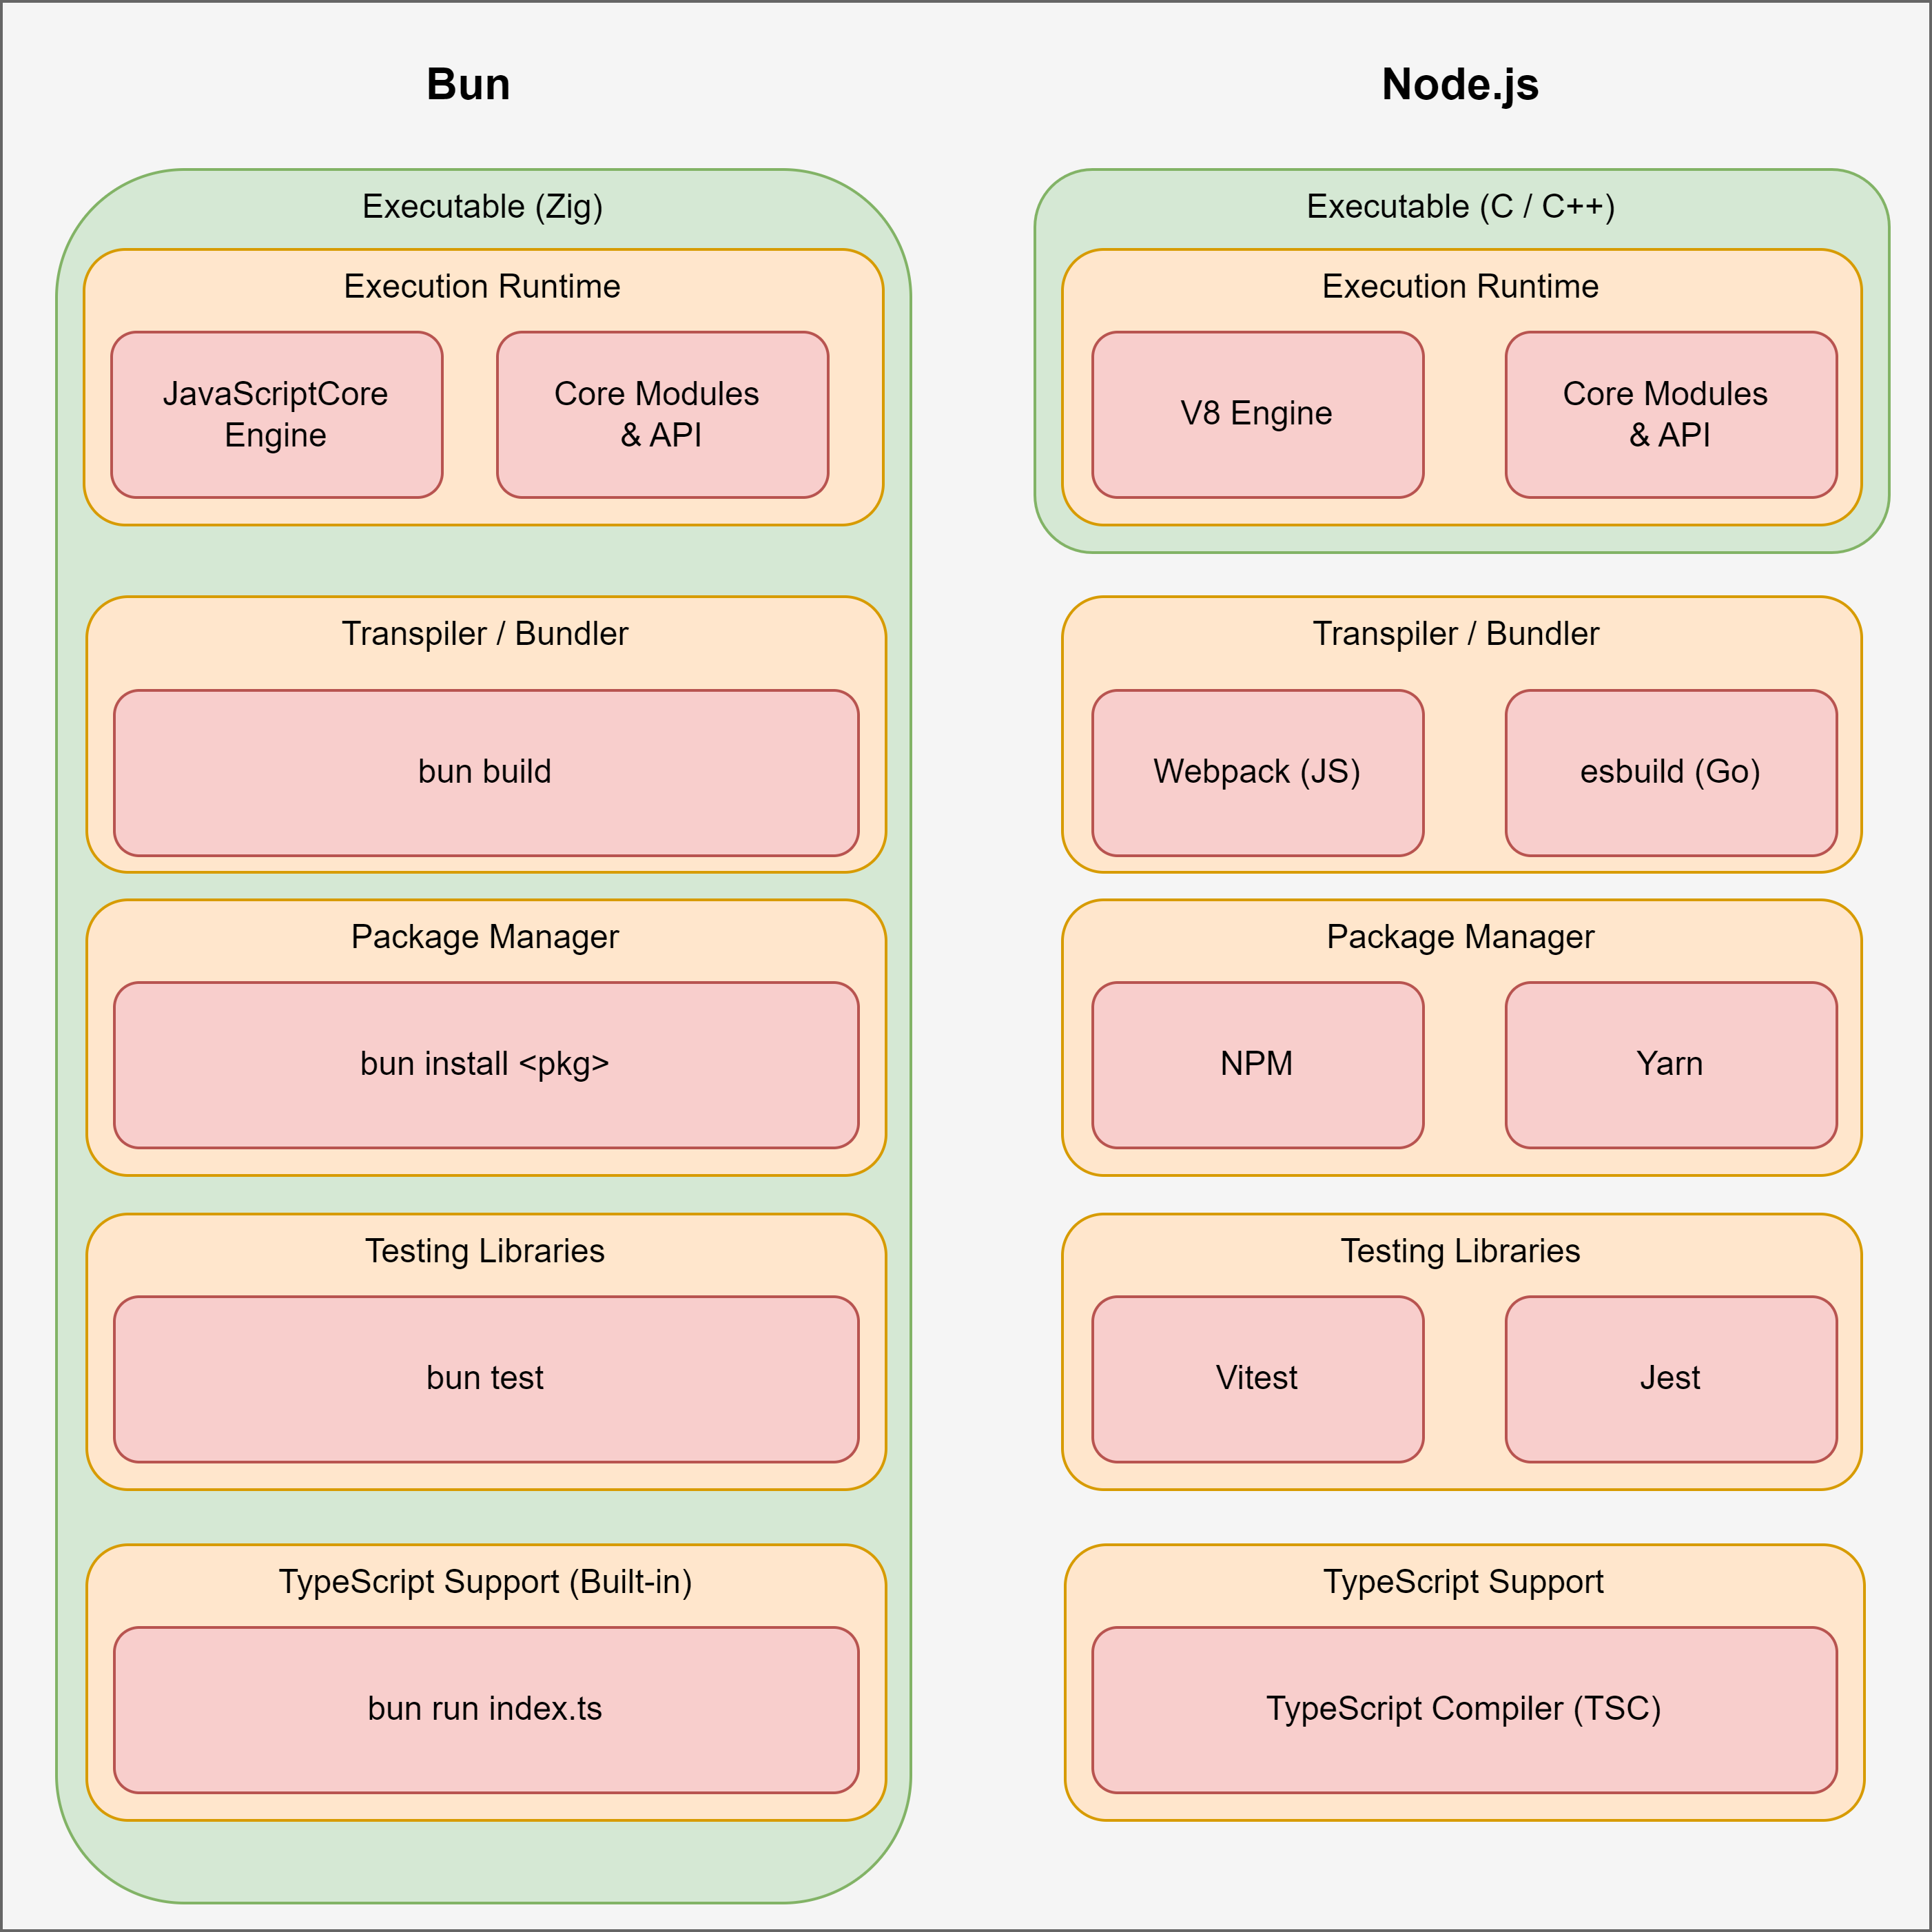
\includegraphics[width=\linewidth]{./images/EcosystemBunvsNode.png}
	\caption{Vergleich der Ökosysteme von Bun und Node.js}
	\label{fig:ecosystemComparison}
	\textit{Quelle: in Anlehnung an \cite{Springer.2022, OvenSh.2023c}}
\end{figure}

\noindent
\autoref{fig:ecosystemComparison} \todo{Markus fragen, ob Verschieben der Absätze verkraftbar ist} zeigt das Ökosystem von Bun im Vergleich zu Node.js. Im Toolkit von Bun sind folgende Komponenten enthalten:
\begin{itemize}
	\item eine Laufzeitumgebung für JavaScript,
	\item ein Paketmanager wie \ac{npm} (siehe \autoref{sec:foundations-Node.js}) oder Yarn, 
	\item ein Transpiler wie Babel,
	\item ein Build-Tool wie Webpack,
	\item Bibliotheken zum Testen wie Jest oder Vitest,
	\item und integrierte Unterstützung für TypeScript \cite{Sumner.2023c}.
\end{itemize}

\noindent
Bun strebt an, das Rundum-sorglos-Tool zu sein, damit alle benötigten Funktionalitäten im Kontext von JavaScript nativ verfügbar sind. Gleichzeitig sollen dadurch die Abhängigkeiten einer Software auf Basis von Bun reduziert werden. In Node.js ist nur die Laufzeitumgebung enthalten, die anderen Komponenten müssen separat installiert werden. Dies bietet allerdings mehr Flexibilität bei der Auswahl der gewünschten Tools.\cite{Springer.2022, OvenSh.2023c}\\

\noindent
Bun ist in Zig geschrieben. Dies ist eine systemnahe Programmiersprache wie C und C++, die sich vor allem auf Einfachheit und Klarheit für ein besseres Verständnis konzentriert \cite{ZigSoftwareFoundation.o.J.}. Die Entwickler haben sich aufgrund der sehr guten Performance und des Speichermanagements für Zig entschieden. Zig ermöglicht mit dessen manuellem Speichermanagement, Klarheit im Kontrollfluss und Klarheit beim Allokieren von Speicher weitere Verbesserungen der Effizienz. Anstatt der V8 JavaScript Engine von Google verwendet Bun die JavaScriptCore Engine. Das ist die Engine für WebKit, die unter anderem in Apple's Safari-Browser genutzt wird. In Kombination mit Zig sorgt die JavaScriptCore Engine für eine bessere Performance und zu reduzierten Startzeiten. Dies ist auf die Architektur der JavaScriptCore Engine mit drei \ac{jit-compiler-dativ-plural} zurückzuführen. Dadurch kann die Engine den Quellcode besser optimieren. Das ist vor allem im Bereich des Serverless Computing ein Vorteil gegenüber anderen Alternativen. Die niedrigen Startzeiten helfen die Skalierbarkeit einer Software zu verbessern, indem neue Knoten schneller hinzugezogen werden können.\cite{OvenSh.2023c, OvenSh.2022, Apple.o.J., Apple.o.J.b, Silva.2020}

\noindent
Node.js bietet viele Module, globale Objekte und Standard-Web-APIs an (siehe \autoref{sec:foundations-Node.js}). Bun möchte eine nahtlose Integration mit Node.js anbieten. Dazu haben die Entwickler verbesserte Versionen für viele dieser Objekte implementiert. Hierzu zählen beispielsweise:
\begin{itemize}
	\item Standard-Web-API: \textit{fetch}, \textit{Request}, \textit{Response},
	\item Module: \text{http}, \text{https}, \text{path},
	\item Globale Objekte: \text{btoa} (Binary to ASCII), \textit{atob} (ASCII to Binary).\cite{OvenSh.2023c}
\end{itemize} 

\noindent
Allerdings existieren auch viele Module und globale Objekte, für die die Unterstützung teilweise oder komplett fehlen, zum Beispiel \textit{tel}, \textit{net} oder \textit{http2} \cite{OvenSh.2023c}. Daraus folgt, dass die Kompatibilität von bestehenden Node.js-Projekten von den verwendeten Objekten und Modulen abhängt.

\section{Performance als Qualitätsattribut} \label{sec:foundations-Performance}
Um eine qualitativ hochwertige Software zu entwickeln, genügt es nicht, die funktionalen Anforderungen zu erfüllen. Entwickler tragen die Verantwortung, die Anforderungen an eine Applikation, sowohl die funktionalen als auch die nichtfunktionalen Aspekte, in vollem Umfang zu erfüllen. Die Qualität einer Software besteht darin, in welchem Maße die Software die expliziten und impliziten Bedürfnisse seiner Stakeholder zufriedenstellt und so Mehrwehrt bietet. Diese Bedürfnisse werden im Qualitätsmodell nach ISO / IEC 25010:2011 dargestellt.\cite{.2022}\\

\begin{figure}[h]
	\centering
	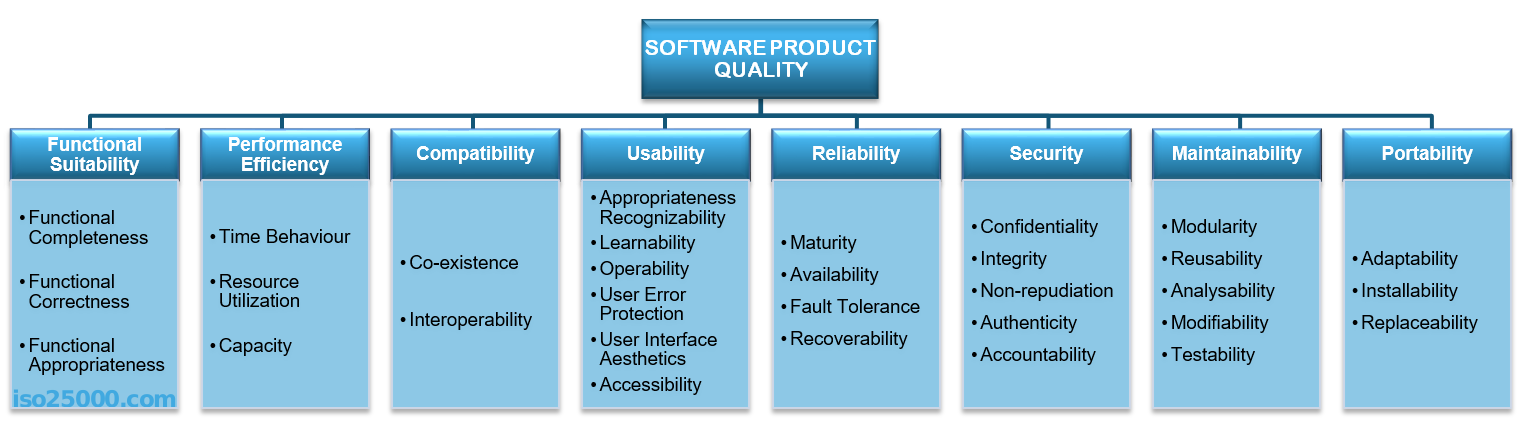
\includegraphics[width=\linewidth]{./images/iso25010.png}
	\caption{Qualitätsattribute einer Software}
	\label{fig:softwareQuality}
	\textit{Quelle: \cite{.2022}}
\end{figure}

\noindent
\autoref{fig:softwareQuality} zeigt die acht Charakteristika der Software-Qualität nach ISO / IEC 25010: Funktionalität, Performance, Kompatibilität, Benutzbarkeit, Zuverlässigkeit, Sicherheit, Wartbarkeit und Portierbarkeit. Der Standard bietet ein Framework für die Bewertung der Qualität einer Software an. Er hilft so Software-Produkte zu verbessern und alle Teilbereiche zu beachten, indem der Standard als Leitfaden vom Identifizieren der Anforderungen bis zur Qualitätskontrolle der Software unterstützt.\cite{ISOIEC.}\\

\noindent
Performance definiert sich im IEEE Standard Glossary of Software Engineering Terminology wie folgt:
\begin{quote}
	\emph{\grqq{}The degree to which a system or component accomplishes its designated functions within given constraints, such as speed, accuracy, or memory usage\grqq{}} \cite{IEEE.}
\end{quote}

\noindent
Demnach beschreibt Performance die Reaktion eines Systems auf die Durchführung einer Aktion über einen definierten Zeitraum. Um die Performance einer Software bestimmen zu können, stellt ISO / IEC 25010 drei Charakteristiken zur Verfügung (siehe \autoref{fig:softwareQuality}), die in den folgenden Absätzen beschrieben werden.\\

\noindent
\textbf{Zeitverhalten}\newline
Das Zeitverhalten beschreibt das Maß, in dem die Reaktions-, Verarbeitungszeiten und Durchsatzraten eines Software-Produkts bei der Ausführung definierten Anforderungen entsprechen \cite{ISOIEC.}. Der Fokus liegt hier auf einer schnellen Reaktion der Software, um die definierten Vorgaben für die Performance einzuhalten. Das Zeitverhalten kann durch die Latenz und den Durchsatz genauer spezifiziert werden. Die Latenz definiert einen zeitlichen Intervall, in dem die Software eine Antwort auf die Anfrage liefern muss. Dieses Intervall wird in einem Zeitfenster durch eine minimale und maximale Zeitangabe definiert. Die Zeitangaben können absolut oder relativ in Bezug auf ein Event angegeben werden. Die Anzahl an abgeschlossenen Antworten auf eine Anfrage innerhalb eines Beobachtungsintervalls beschreibt den Durchsatz. Dadurch kann die Verarbeitungsleistung (Processing Rate) der Software abgeleitet werden. Für eine zuverlässige Angabe ist es empfohlen, mehrere Zeitfenster zu beobachten. Denn es kann sein, dass eine Software 120 Anfragen innerhalb 1 Stunde bearbeiten kann. Dennoch könnte das System versagen, wenn 40 dieser Anfragen innerhalb von 3 Minuten abgearbeitet werden müssen.\cite{Barbacci.1995}\\

\noindent
\textbf{Ressourcennutzung}\newline
Das Maß, in dem die Menge und Art der Ressource, die ein Produkt bei der Ausführung seiner Funktionalitäten beansprucht, entspricht der Ressourcennutzung \cite{ISOIEC.}. Es geht um die effiziente Verwaltung der verfügbaren Ressourcen. Dazu zählen die CPU, der Arbeitsspeicher, die Bandbreite des Netzwerks, der Speicherplatz auf der Festplatte und viele mehr. Die wichtigsten Metriken sind die CPU-Auslastung, der Speicherbedarf sowohl im RAM als auch auf der Festplatte.\cite{Barbacci.1995}\\

\noindent
\textbf{Kapazität}\newline
Die Kapazität entspricht dem Maß, in dem die maximalen Grenzen eines Parameters einer Software den Anforderungen entsprechen \cite{ISOIEC.}. Dadurch wird bestimmt, ob das System unter Spitzenlast funktionsfähig bleibt und dadurch skalierbar ist. Hierbei müssen die Anforderungen an die maximale Latenz eingehalten werden. Daher kann die Kapazität alternativ auch als der maximal mögliche Durchsatz unter Einhaltung der gegebenen Latenzanforderungen bezeichnet werden. Das umfasst mehrere Benutzer, die gleichzeitig auf die Software zugreifen, oder größere Transaktionen mit mehr Datenvolumen. Zu den Metriken zählen die maximale Anzahl an gleichzeitigen Benutzern und die maximale Anzahl an möglichen Transaktionen.\cite{Barbacci.1995}